\documentclass[border=3pt]{standalone}
% Shared TikZ styles for all paper figures.
%
% Colour is used to separate the two views (logical = blue, physical = ochre)
% and to mark the one emphasised relation (rose). Shape, line style and weight
% carry the same distinctions independently, so the figures still read when
% printed in black and white -- see the greyscale check in `make gray`.
\usepackage{tikz}
\usepackage{amsmath}
\usepackage[scaled=0.92]{helvet}
\renewcommand{\familydefault}{\sfdefault}
% Define \GRAYFIGS before % Shared TikZ styles for all paper figures.
%
% Colour is used to separate the two views (logical = blue, physical = ochre)
% and to mark the one emphasised relation (rose). Shape, line style and weight
% carry the same distinctions independently, so the figures still read when
% printed in black and white -- see the greyscale check in `make gray`.
\usepackage{tikz}
\usepackage{amsmath}
\usepackage[scaled=0.92]{helvet}
\renewcommand{\familydefault}{\sfdefault}
% Define \GRAYFIGS before % Shared TikZ styles for all paper figures.
%
% Colour is used to separate the two views (logical = blue, physical = ochre)
% and to mark the one emphasised relation (rose). Shape, line style and weight
% carry the same distinctions independently, so the figures still read when
% printed in black and white -- see the greyscale check in `make gray`.
\usepackage{tikz}
\usepackage{amsmath}
\usepackage[scaled=0.92]{helvet}
\renewcommand{\familydefault}{\sfdefault}
% Define \GRAYFIGS before \input{figstyle} to build the same figures in
% greyscale (xcolor converts every colour below), e.g.
%   pdflatex -jobname=fig1_gray "\def\GRAYFIGS{}\input{fig1_concept}"
\ifdefined\GRAYFIGS
  \usepackage[gray]{xcolor}
\else
  \usepackage{xcolor}
\fi
\usetikzlibrary{arrows.meta,positioning,fit,backgrounds,calc,shapes.geometric,
                shapes.misc,decorations.pathreplacing,patterns,matrix,shadows.blur}

% ------------------------------- palette -----------------------------------
\definecolor{ink}{HTML}{22333F}        % primary text
\definecolor{inkSoft}{HTML}{6B8299}    % secondary text, hairlines
\definecolor{astLine}{HTML}{2C7A9B}    % logical view
\definecolor{astFill}{HTML}{E7F2F7}
\definecolor{pdfLine}{HTML}{B0762F}    % physical view
\definecolor{pdfFill}{HTML}{FBF2E3}
\definecolor{hotLine}{HTML}{B03A55}    % the emphasised relation
\definecolor{hotFill}{HTML}{FBE9EC}
\definecolor{mutedLine}{HTML}{9FB3C8}  % furniture / unmatched
\definecolor{mutedFill}{HTML}{F1F5F8}

\tikzset{
  every node/.append style = {text=ink},
  >=Stealth,
  % --- logical structure (AST) -------------------------------------------
  astnode/.style   = {draw=astLine!70, fill=white, rounded corners=2.5pt,
                      line width=0.6pt, font=\scriptsize,
                      inner xsep=4pt, inner ysep=2.5pt, minimum height=4.6mm},
  astroot/.style   = {astnode, fill=astLine, draw=astLine, text=white},
  astsec/.style    = {astnode, fill=astFill},
  asttree/.style   = {draw=astLine!50, line width=0.6pt, rounded corners=2.5pt},
  % --- physical layout (page regions) ------------------------------------
  page/.style      = {draw=inkSoft!45, fill=white, line width=0.6pt,
                      rounded corners=2pt},
  lbox/.style      = {draw=pdfLine!55, fill=white, line width=0.6pt,
                      rounded corners=1.2pt},
  lboxhi/.style    = {draw=hotLine, fill=hotFill, line width=1.0pt,
                      rounded corners=1.2pt},
  furniture/.style = {draw=mutedLine, dash pattern=on 1.6pt off 1.4pt,
                      fill=mutedFill, line width=0.6pt, rounded corners=1.2pt},
  % --- relations ----------------------------------------------------------
  maplink/.style   = {draw=inkSoft, line width=0.6pt,
                      -{Stealth[length=1.7mm,width=1.3mm]}},
  maphot/.style    = {draw=hotLine, line width=1.1pt,
                      -{Stealth[length=2mm,width=1.6mm]}},
  flow/.style      = {draw=inkSoft, line width=0.7pt,
                      -{Stealth[length=2mm,width=1.6mm]}, rounded corners=2pt},
  % --- pipeline stages ----------------------------------------------------
  stage/.style     = {draw=inkSoft!55, fill=white, rounded corners=2.5pt,
                      font=\scriptsize, align=center, inner sep=3.5pt,
                      minimum height=7mm, text width=32mm},
  artefact/.style  = {draw=inkSoft!35, fill=mutedFill, rounded corners=2.5pt,
                      font=\scriptsize, align=center, inner sep=3.5pt,
                      minimum height=7mm, text width=32mm},
  % --- labels -------------------------------------------------------------
  grouplbl/.style  = {font=\scriptsize, text=inkSoft},
  caption/.style   = {font=\scriptsize, text=ink},
  tinylbl/.style   = {font=\tiny, text=inkSoft},
  softcard/.style  = {rounded corners=4pt, draw=none},
}

% Fake text lines inside a layout box.
% [colour] {x} {y top} {width} {line count}
\newcommand{\fakelines}[5][pdfLine!32]{%
  \foreach \fli in {1,...,#5}{%
    \draw[#1, line width=0.32pt] (#2,{#3-0.115*\fli}) -- ++({#4},0);}%
}
% Same, with a short final line (end of a paragraph)
\newcommand{\fakepara}[5][pdfLine!32]{%
  \foreach \fli in {1,...,#5}{%
    \draw[#1, line width=0.32pt] (#2,{#3-0.115*\fli}) -- ++({#4},0);}%
  \draw[#1, line width=0.32pt] (#2,{#3-0.115*(#5+1)}) -- ++({0.55*#4},0);%
}
 to build the same figures in
% greyscale (xcolor converts every colour below), e.g.
%   pdflatex -jobname=fig1_gray "\def\GRAYFIGS{}\documentclass[border=3pt]{standalone}
\input{figstyle}
\begin{document}
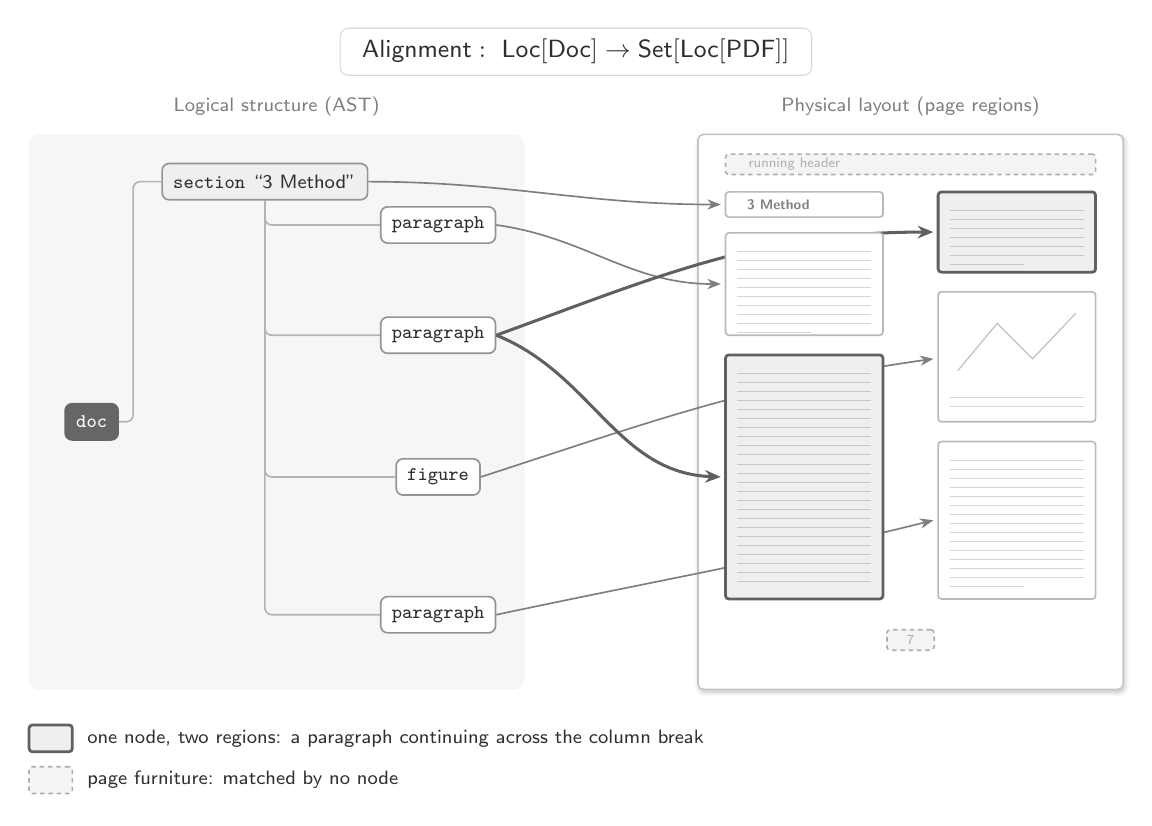
\begin{tikzpicture}

% ============================ title badge ==================================
\node[rounded corners=3pt, draw=inkSoft!30, fill=white, inner xsep=8pt,
      inner ysep=4pt, font=\small] at (6.95,8.00)
     {$\mathsf{Alignment}:\ \mathsf{Loc}[\mathsf{Doc}] \rightarrow
       \mathsf{Set}[\mathsf{Loc}[\mathsf{PDF}]]$};

\node[grouplbl] at (3.15,7.30) {Logical structure (AST)};
\node[grouplbl] at (11.20,7.30) {Physical layout (page regions)};

% ============================ the two cards ================================
\fill[softcard, fill=astFill!55] (0.00,-0.10) rectangle (6.30,6.95);
\node[page, fit={(8.50,-0.10) (13.90,6.95)}, inner sep=0pt,
      blur shadow={shadow blur steps=8, shadow xshift=0.5pt,
                   shadow yshift=-0.9pt, shadow opacity=25}] {};

% ======================= LEFT: logical structure (AST) =====================
\node[astroot] (doc)  at (0.80,3.30) {\texttt{doc}};
\node[astsec]  (sec1) at (3.00,6.35) {\texttt{section} ``3 Method''};
\node[astnode] (p1)   at (5.20,5.80) {\texttt{paragraph}};
\node[astnode] (p2)   at (5.20,4.40) {\texttt{paragraph}};
\node[astnode] (fg)   at (5.20,2.60) {\texttt{figure}};
\node[astnode] (p3)   at (5.20,0.85) {\texttt{paragraph}};

\draw[asttree] (doc.east) -- ++(0.18,0) |- (sec1.west);
\foreach \c in {p1,p2,fg,p3}{ \draw[asttree] (sec1.south) |- (\c.west); }

% ============================= THE MAPPING =================================
% (drawn before the regions, so the links pass behind them)
\draw[maplink] (sec1.east) to[out=0,in=180]   (8.79,6.06);
\draw[maplink] (p1.east)   to[out=-8,in=180]  (8.79,5.05);
\draw[maplink] (fg.east)   to[out=18,in=188]  (11.49,4.10);
\draw[maplink] (p3.east)   to[out=12,in=194]  (11.49,2.05);

% one node, two regions, split across the column break
\draw[maphot]  (p2.east) to[out=-22,in=178] (8.79,2.60);
\draw[maphot]  (p2.east) to[out=20,in=180]  (11.49,5.71);

% ======================= page regions (opaque, on top) =====================
\node[furniture, fit={(8.85,6.44) (13.55,6.70)}, inner sep=0pt] {};
\node[font=\tiny, text=mutedLine, anchor=west] at (9.02,6.57) {running header};
\node[furniture, fit={(10.90,0.40) (11.50,0.66)}, inner sep=0pt] {};
\node[font=\tiny, text=mutedLine] at (11.20,0.53) {7};

% --- left column ---
\node[lbox, fit={(8.85,5.90) (10.85,6.22)}, inner sep=0pt] {};
\node[font=\tiny, text=pdfLine, anchor=west] at (9.00,6.06) {\textbf{3 Method}};

\node[lbox, fit={(8.85,4.40) (10.85,5.70)}, inner sep=0pt] {};
\fakepara{9.00}{5.58}{1.70}{9}

\node[lboxhi, fit={(8.85,1.05) (10.85,4.15)}, inner sep=0pt] {};
\fakelines[hotLine!35]{9.00}{4.03}{1.70}{24}

% --- right column ---
\node[lboxhi, fit={(11.55,5.20) (13.55,6.22)}, inner sep=0pt] {};
\fakepara[hotLine!35]{11.70}{6.10}{1.70}{6}

\node[lbox, fit={(11.55,3.30) (13.55,4.95)}, inner sep=0pt] {};
\draw[pdfLine!45, line width=0.5pt, line join=round]
      (11.80,3.95) -- (12.30,4.55) -- (12.75,4.10) -- (13.30,4.68);
\fakelines{11.70}{3.72}{1.70}{2}

\node[lbox, fit={(11.55,1.05) (13.55,3.05)}, inner sep=0pt] {};
\fakepara{11.70}{2.93}{1.70}{14}

% ================================ legend ===================================
\node[lboxhi, minimum width=5.5mm, minimum height=3.4mm, inner sep=0pt]
      at (0.28,-0.72) {};
\node[caption, anchor=west] at (0.62,-0.72)
     {one node, two regions: a paragraph continuing across the column break};

\node[furniture, minimum width=5.5mm, minimum height=3.4mm, inner sep=0pt]
      at (0.28,-1.25) {};
\node[caption, anchor=west] at (0.62,-1.25)
     {page furniture: matched by no node};

\end{tikzpicture}
\end{document}
"
\ifdefined\GRAYFIGS
  \usepackage[gray]{xcolor}
\else
  \usepackage{xcolor}
\fi
\usetikzlibrary{arrows.meta,positioning,fit,backgrounds,calc,shapes.geometric,
                shapes.misc,decorations.pathreplacing,patterns,matrix,shadows.blur}

% ------------------------------- palette -----------------------------------
\definecolor{ink}{HTML}{22333F}        % primary text
\definecolor{inkSoft}{HTML}{6B8299}    % secondary text, hairlines
\definecolor{astLine}{HTML}{2C7A9B}    % logical view
\definecolor{astFill}{HTML}{E7F2F7}
\definecolor{pdfLine}{HTML}{B0762F}    % physical view
\definecolor{pdfFill}{HTML}{FBF2E3}
\definecolor{hotLine}{HTML}{B03A55}    % the emphasised relation
\definecolor{hotFill}{HTML}{FBE9EC}
\definecolor{mutedLine}{HTML}{9FB3C8}  % furniture / unmatched
\definecolor{mutedFill}{HTML}{F1F5F8}

\tikzset{
  every node/.append style = {text=ink},
  >=Stealth,
  % --- logical structure (AST) -------------------------------------------
  astnode/.style   = {draw=astLine!70, fill=white, rounded corners=2.5pt,
                      line width=0.6pt, font=\scriptsize,
                      inner xsep=4pt, inner ysep=2.5pt, minimum height=4.6mm},
  astroot/.style   = {astnode, fill=astLine, draw=astLine, text=white},
  astsec/.style    = {astnode, fill=astFill},
  asttree/.style   = {draw=astLine!50, line width=0.6pt, rounded corners=2.5pt},
  % --- physical layout (page regions) ------------------------------------
  page/.style      = {draw=inkSoft!45, fill=white, line width=0.6pt,
                      rounded corners=2pt},
  lbox/.style      = {draw=pdfLine!55, fill=white, line width=0.6pt,
                      rounded corners=1.2pt},
  lboxhi/.style    = {draw=hotLine, fill=hotFill, line width=1.0pt,
                      rounded corners=1.2pt},
  furniture/.style = {draw=mutedLine, dash pattern=on 1.6pt off 1.4pt,
                      fill=mutedFill, line width=0.6pt, rounded corners=1.2pt},
  % --- relations ----------------------------------------------------------
  maplink/.style   = {draw=inkSoft, line width=0.6pt,
                      -{Stealth[length=1.7mm,width=1.3mm]}},
  maphot/.style    = {draw=hotLine, line width=1.1pt,
                      -{Stealth[length=2mm,width=1.6mm]}},
  flow/.style      = {draw=inkSoft, line width=0.7pt,
                      -{Stealth[length=2mm,width=1.6mm]}, rounded corners=2pt},
  % --- pipeline stages ----------------------------------------------------
  stage/.style     = {draw=inkSoft!55, fill=white, rounded corners=2.5pt,
                      font=\scriptsize, align=center, inner sep=3.5pt,
                      minimum height=7mm, text width=32mm},
  artefact/.style  = {draw=inkSoft!35, fill=mutedFill, rounded corners=2.5pt,
                      font=\scriptsize, align=center, inner sep=3.5pt,
                      minimum height=7mm, text width=32mm},
  % --- labels -------------------------------------------------------------
  grouplbl/.style  = {font=\scriptsize, text=inkSoft},
  caption/.style   = {font=\scriptsize, text=ink},
  tinylbl/.style   = {font=\tiny, text=inkSoft},
  softcard/.style  = {rounded corners=4pt, draw=none},
}

% Fake text lines inside a layout box.
% [colour] {x} {y top} {width} {line count}
\newcommand{\fakelines}[5][pdfLine!32]{%
  \foreach \fli in {1,...,#5}{%
    \draw[#1, line width=0.32pt] (#2,{#3-0.115*\fli}) -- ++({#4},0);}%
}
% Same, with a short final line (end of a paragraph)
\newcommand{\fakepara}[5][pdfLine!32]{%
  \foreach \fli in {1,...,#5}{%
    \draw[#1, line width=0.32pt] (#2,{#3-0.115*\fli}) -- ++({#4},0);}%
  \draw[#1, line width=0.32pt] (#2,{#3-0.115*(#5+1)}) -- ++({0.55*#4},0);%
}
 to build the same figures in
% greyscale (xcolor converts every colour below), e.g.
%   pdflatex -jobname=fig1_gray "\def\GRAYFIGS{}\documentclass[border=3pt]{standalone}
% Shared TikZ styles for all paper figures.
%
% Colour is used to separate the two views (logical = blue, physical = ochre)
% and to mark the one emphasised relation (rose). Shape, line style and weight
% carry the same distinctions independently, so the figures still read when
% printed in black and white -- see the greyscale check in `make gray`.
\usepackage{tikz}
\usepackage{amsmath}
\usepackage[scaled=0.92]{helvet}
\renewcommand{\familydefault}{\sfdefault}
% Define \GRAYFIGS before \input{figstyle} to build the same figures in
% greyscale (xcolor converts every colour below), e.g.
%   pdflatex -jobname=fig1_gray "\def\GRAYFIGS{}\input{fig1_concept}"
\ifdefined\GRAYFIGS
  \usepackage[gray]{xcolor}
\else
  \usepackage{xcolor}
\fi
\usetikzlibrary{arrows.meta,positioning,fit,backgrounds,calc,shapes.geometric,
                shapes.misc,decorations.pathreplacing,patterns,matrix,shadows.blur}

% ------------------------------- palette -----------------------------------
\definecolor{ink}{HTML}{22333F}        % primary text
\definecolor{inkSoft}{HTML}{6B8299}    % secondary text, hairlines
\definecolor{astLine}{HTML}{2C7A9B}    % logical view
\definecolor{astFill}{HTML}{E7F2F7}
\definecolor{pdfLine}{HTML}{B0762F}    % physical view
\definecolor{pdfFill}{HTML}{FBF2E3}
\definecolor{hotLine}{HTML}{B03A55}    % the emphasised relation
\definecolor{hotFill}{HTML}{FBE9EC}
\definecolor{mutedLine}{HTML}{9FB3C8}  % furniture / unmatched
\definecolor{mutedFill}{HTML}{F1F5F8}

\tikzset{
  every node/.append style = {text=ink},
  >=Stealth,
  % --- logical structure (AST) -------------------------------------------
  astnode/.style   = {draw=astLine!70, fill=white, rounded corners=2.5pt,
                      line width=0.6pt, font=\scriptsize,
                      inner xsep=4pt, inner ysep=2.5pt, minimum height=4.6mm},
  astroot/.style   = {astnode, fill=astLine, draw=astLine, text=white},
  astsec/.style    = {astnode, fill=astFill},
  asttree/.style   = {draw=astLine!50, line width=0.6pt, rounded corners=2.5pt},
  % --- physical layout (page regions) ------------------------------------
  page/.style      = {draw=inkSoft!45, fill=white, line width=0.6pt,
                      rounded corners=2pt},
  lbox/.style      = {draw=pdfLine!55, fill=white, line width=0.6pt,
                      rounded corners=1.2pt},
  lboxhi/.style    = {draw=hotLine, fill=hotFill, line width=1.0pt,
                      rounded corners=1.2pt},
  furniture/.style = {draw=mutedLine, dash pattern=on 1.6pt off 1.4pt,
                      fill=mutedFill, line width=0.6pt, rounded corners=1.2pt},
  % --- relations ----------------------------------------------------------
  maplink/.style   = {draw=inkSoft, line width=0.6pt,
                      -{Stealth[length=1.7mm,width=1.3mm]}},
  maphot/.style    = {draw=hotLine, line width=1.1pt,
                      -{Stealth[length=2mm,width=1.6mm]}},
  flow/.style      = {draw=inkSoft, line width=0.7pt,
                      -{Stealth[length=2mm,width=1.6mm]}, rounded corners=2pt},
  % --- pipeline stages ----------------------------------------------------
  stage/.style     = {draw=inkSoft!55, fill=white, rounded corners=2.5pt,
                      font=\scriptsize, align=center, inner sep=3.5pt,
                      minimum height=7mm, text width=32mm},
  artefact/.style  = {draw=inkSoft!35, fill=mutedFill, rounded corners=2.5pt,
                      font=\scriptsize, align=center, inner sep=3.5pt,
                      minimum height=7mm, text width=32mm},
  % --- labels -------------------------------------------------------------
  grouplbl/.style  = {font=\scriptsize, text=inkSoft},
  caption/.style   = {font=\scriptsize, text=ink},
  tinylbl/.style   = {font=\tiny, text=inkSoft},
  softcard/.style  = {rounded corners=4pt, draw=none},
}

% Fake text lines inside a layout box.
% [colour] {x} {y top} {width} {line count}
\newcommand{\fakelines}[5][pdfLine!32]{%
  \foreach \fli in {1,...,#5}{%
    \draw[#1, line width=0.32pt] (#2,{#3-0.115*\fli}) -- ++({#4},0);}%
}
% Same, with a short final line (end of a paragraph)
\newcommand{\fakepara}[5][pdfLine!32]{%
  \foreach \fli in {1,...,#5}{%
    \draw[#1, line width=0.32pt] (#2,{#3-0.115*\fli}) -- ++({#4},0);}%
  \draw[#1, line width=0.32pt] (#2,{#3-0.115*(#5+1)}) -- ++({0.55*#4},0);%
}

\begin{document}
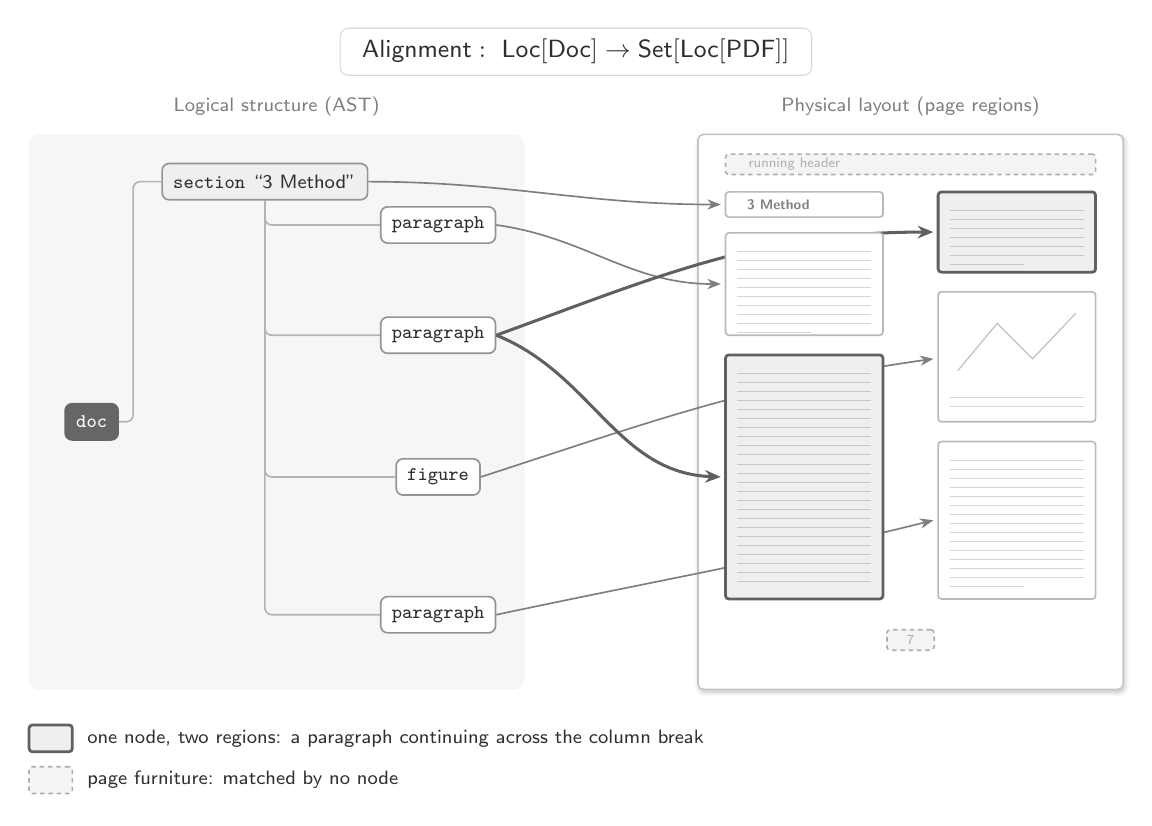
\begin{tikzpicture}

% ============================ title badge ==================================
\node[rounded corners=3pt, draw=inkSoft!30, fill=white, inner xsep=8pt,
      inner ysep=4pt, font=\small] at (6.95,8.00)
     {$\mathsf{Alignment}:\ \mathsf{Loc}[\mathsf{Doc}] \rightarrow
       \mathsf{Set}[\mathsf{Loc}[\mathsf{PDF}]]$};

\node[grouplbl] at (3.15,7.30) {Logical structure (AST)};
\node[grouplbl] at (11.20,7.30) {Physical layout (page regions)};

% ============================ the two cards ================================
\fill[softcard, fill=astFill!55] (0.00,-0.10) rectangle (6.30,6.95);
\node[page, fit={(8.50,-0.10) (13.90,6.95)}, inner sep=0pt,
      blur shadow={shadow blur steps=8, shadow xshift=0.5pt,
                   shadow yshift=-0.9pt, shadow opacity=25}] {};

% ======================= LEFT: logical structure (AST) =====================
\node[astroot] (doc)  at (0.80,3.30) {\texttt{doc}};
\node[astsec]  (sec1) at (3.00,6.35) {\texttt{section} ``3 Method''};
\node[astnode] (p1)   at (5.20,5.80) {\texttt{paragraph}};
\node[astnode] (p2)   at (5.20,4.40) {\texttt{paragraph}};
\node[astnode] (fg)   at (5.20,2.60) {\texttt{figure}};
\node[astnode] (p3)   at (5.20,0.85) {\texttt{paragraph}};

\draw[asttree] (doc.east) -- ++(0.18,0) |- (sec1.west);
\foreach \c in {p1,p2,fg,p3}{ \draw[asttree] (sec1.south) |- (\c.west); }

% ============================= THE MAPPING =================================
% (drawn before the regions, so the links pass behind them)
\draw[maplink] (sec1.east) to[out=0,in=180]   (8.79,6.06);
\draw[maplink] (p1.east)   to[out=-8,in=180]  (8.79,5.05);
\draw[maplink] (fg.east)   to[out=18,in=188]  (11.49,4.10);
\draw[maplink] (p3.east)   to[out=12,in=194]  (11.49,2.05);

% one node, two regions, split across the column break
\draw[maphot]  (p2.east) to[out=-22,in=178] (8.79,2.60);
\draw[maphot]  (p2.east) to[out=20,in=180]  (11.49,5.71);

% ======================= page regions (opaque, on top) =====================
\node[furniture, fit={(8.85,6.44) (13.55,6.70)}, inner sep=0pt] {};
\node[font=\tiny, text=mutedLine, anchor=west] at (9.02,6.57) {running header};
\node[furniture, fit={(10.90,0.40) (11.50,0.66)}, inner sep=0pt] {};
\node[font=\tiny, text=mutedLine] at (11.20,0.53) {7};

% --- left column ---
\node[lbox, fit={(8.85,5.90) (10.85,6.22)}, inner sep=0pt] {};
\node[font=\tiny, text=pdfLine, anchor=west] at (9.00,6.06) {\textbf{3 Method}};

\node[lbox, fit={(8.85,4.40) (10.85,5.70)}, inner sep=0pt] {};
\fakepara{9.00}{5.58}{1.70}{9}

\node[lboxhi, fit={(8.85,1.05) (10.85,4.15)}, inner sep=0pt] {};
\fakelines[hotLine!35]{9.00}{4.03}{1.70}{24}

% --- right column ---
\node[lboxhi, fit={(11.55,5.20) (13.55,6.22)}, inner sep=0pt] {};
\fakepara[hotLine!35]{11.70}{6.10}{1.70}{6}

\node[lbox, fit={(11.55,3.30) (13.55,4.95)}, inner sep=0pt] {};
\draw[pdfLine!45, line width=0.5pt, line join=round]
      (11.80,3.95) -- (12.30,4.55) -- (12.75,4.10) -- (13.30,4.68);
\fakelines{11.70}{3.72}{1.70}{2}

\node[lbox, fit={(11.55,1.05) (13.55,3.05)}, inner sep=0pt] {};
\fakepara{11.70}{2.93}{1.70}{14}

% ================================ legend ===================================
\node[lboxhi, minimum width=5.5mm, minimum height=3.4mm, inner sep=0pt]
      at (0.28,-0.72) {};
\node[caption, anchor=west] at (0.62,-0.72)
     {one node, two regions: a paragraph continuing across the column break};

\node[furniture, minimum width=5.5mm, minimum height=3.4mm, inner sep=0pt]
      at (0.28,-1.25) {};
\node[caption, anchor=west] at (0.62,-1.25)
     {page furniture: matched by no node};

\end{tikzpicture}
\end{document}
"
\ifdefined\GRAYFIGS
  \usepackage[gray]{xcolor}
\else
  \usepackage{xcolor}
\fi
\usetikzlibrary{arrows.meta,positioning,fit,backgrounds,calc,shapes.geometric,
                shapes.misc,decorations.pathreplacing,patterns,matrix,shadows.blur}

% ------------------------------- palette -----------------------------------
\definecolor{ink}{HTML}{22333F}        % primary text
\definecolor{inkSoft}{HTML}{6B8299}    % secondary text, hairlines
\definecolor{astLine}{HTML}{2C7A9B}    % logical view
\definecolor{astFill}{HTML}{E7F2F7}
\definecolor{pdfLine}{HTML}{B0762F}    % physical view
\definecolor{pdfFill}{HTML}{FBF2E3}
\definecolor{hotLine}{HTML}{B03A55}    % the emphasised relation
\definecolor{hotFill}{HTML}{FBE9EC}
\definecolor{mutedLine}{HTML}{9FB3C8}  % furniture / unmatched
\definecolor{mutedFill}{HTML}{F1F5F8}

\tikzset{
  every node/.append style = {text=ink},
  >=Stealth,
  % --- logical structure (AST) -------------------------------------------
  astnode/.style   = {draw=astLine!70, fill=white, rounded corners=2.5pt,
                      line width=0.6pt, font=\scriptsize,
                      inner xsep=4pt, inner ysep=2.5pt, minimum height=4.6mm},
  astroot/.style   = {astnode, fill=astLine, draw=astLine, text=white},
  astsec/.style    = {astnode, fill=astFill},
  asttree/.style   = {draw=astLine!50, line width=0.6pt, rounded corners=2.5pt},
  % --- physical layout (page regions) ------------------------------------
  page/.style      = {draw=inkSoft!45, fill=white, line width=0.6pt,
                      rounded corners=2pt},
  lbox/.style      = {draw=pdfLine!55, fill=white, line width=0.6pt,
                      rounded corners=1.2pt},
  lboxhi/.style    = {draw=hotLine, fill=hotFill, line width=1.0pt,
                      rounded corners=1.2pt},
  furniture/.style = {draw=mutedLine, dash pattern=on 1.6pt off 1.4pt,
                      fill=mutedFill, line width=0.6pt, rounded corners=1.2pt},
  % --- relations ----------------------------------------------------------
  maplink/.style   = {draw=inkSoft, line width=0.6pt,
                      -{Stealth[length=1.7mm,width=1.3mm]}},
  maphot/.style    = {draw=hotLine, line width=1.1pt,
                      -{Stealth[length=2mm,width=1.6mm]}},
  flow/.style      = {draw=inkSoft, line width=0.7pt,
                      -{Stealth[length=2mm,width=1.6mm]}, rounded corners=2pt},
  % --- pipeline stages ----------------------------------------------------
  stage/.style     = {draw=inkSoft!55, fill=white, rounded corners=2.5pt,
                      font=\scriptsize, align=center, inner sep=3.5pt,
                      minimum height=7mm, text width=32mm},
  artefact/.style  = {draw=inkSoft!35, fill=mutedFill, rounded corners=2.5pt,
                      font=\scriptsize, align=center, inner sep=3.5pt,
                      minimum height=7mm, text width=32mm},
  % --- labels -------------------------------------------------------------
  grouplbl/.style  = {font=\scriptsize, text=inkSoft},
  caption/.style   = {font=\scriptsize, text=ink},
  tinylbl/.style   = {font=\tiny, text=inkSoft},
  softcard/.style  = {rounded corners=4pt, draw=none},
}

% Fake text lines inside a layout box.
% [colour] {x} {y top} {width} {line count}
\newcommand{\fakelines}[5][pdfLine!32]{%
  \foreach \fli in {1,...,#5}{%
    \draw[#1, line width=0.32pt] (#2,{#3-0.115*\fli}) -- ++({#4},0);}%
}
% Same, with a short final line (end of a paragraph)
\newcommand{\fakepara}[5][pdfLine!32]{%
  \foreach \fli in {1,...,#5}{%
    \draw[#1, line width=0.32pt] (#2,{#3-0.115*\fli}) -- ++({#4},0);}%
  \draw[#1, line width=0.32pt] (#2,{#3-0.115*(#5+1)}) -- ++({0.55*#4},0);%
}

\begin{document}
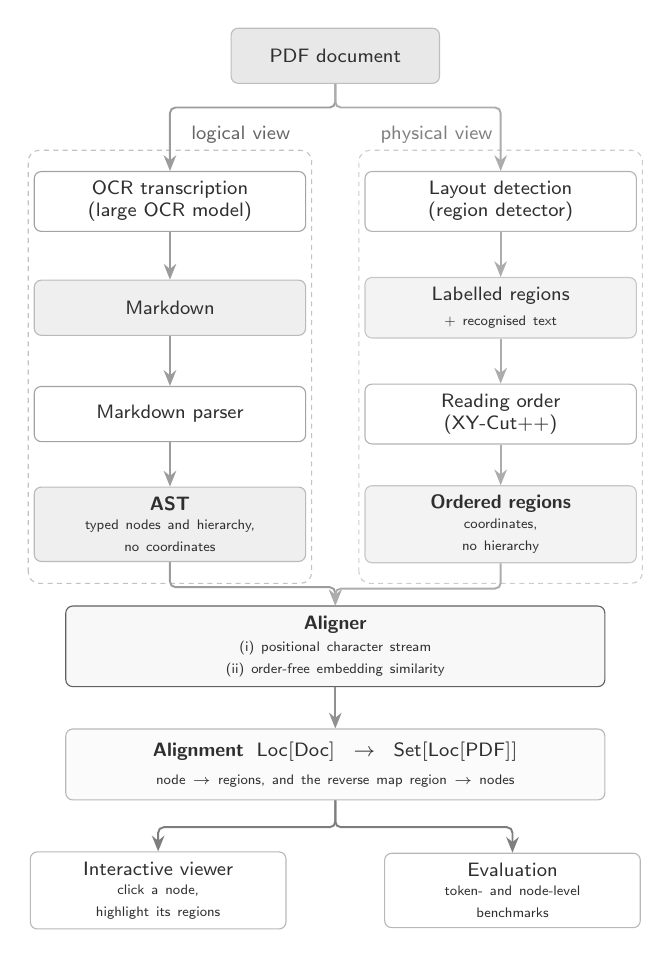
\begin{tikzpicture}[
  lstage/.style = {stage,    draw=astLine!60},
  lart/.style   = {artefact, draw=astLine!45, fill=astFill},
  pstage/.style = {stage,    draw=pdfLine!60},
  part/.style   = {artefact, draw=pdfLine!45, fill=pdfFill},
  lflow/.style  = {flow, draw=astLine!65},
  pflow/.style  = {flow, draw=pdfLine!65},
]

% ------------------------------- input -------------------------------------
\node[artefact, text width=24mm, draw=inkSoft!50, fill=inkSoft!18]
     (pdf) at (4.15,9.05) {PDF document};

% --------------------------- logical branch --------------------------------
\node[lstage] (ocr)  at (2.05,7.20) {OCR transcription\\(large OCR model)};
\node[lart]   (md)   at (2.05,5.85) {Markdown};
\node[lstage] (bast) at (2.05,4.50) {Markdown parser};
\node[lart]   (ast)  at (2.05,3.10)
      {\textbf{AST}\\[1pt]\tiny typed nodes and hierarchy,\\ no coordinates};

% --------------------------- physical branch -------------------------------
\node[pstage] (det)  at (6.25,7.20) {Layout detection\\(region detector)};
\node[part]   (reg)  at (6.25,5.85) {Labelled regions\\[1pt]\tiny + recognised text};
\node[pstage] (ro)   at (6.25,4.50) {Reading order\\(XY-Cut++)};
\node[part]   (box)  at (6.25,3.10)
      {\textbf{Ordered regions}\\[1pt]\tiny coordinates,\\ no hierarchy};

% ------------------------------ aligner ------------------------------------
\node[stage, draw=hotLine, fill=hotFill!45, text width=66mm, minimum height=10mm]
     (al) at (4.15,1.55)
      {\textbf{Aligner}\\[2pt]
       \tiny (i) positional character stream\\
             (ii) order-free embedding similarity};

\node[artefact, draw=hotLine!45, fill=hotFill!25, text width=66mm,
      minimum height=9mm] (out) at (4.15,0.05)
      {\textbf{Alignment}\; $\mathsf{Loc}[\mathsf{Doc}] \rightarrow
       \mathsf{Set}[\mathsf{Loc}[\mathsf{PDF}]]$\\[2pt]
       \tiny node $\rightarrow$ regions, and the reverse map region $\rightarrow$ nodes};

% ----------------------------- consumers -----------------------------------
\node[stage, text width=30mm] (ui) at (1.90,-1.55)
      {Interactive viewer\\[1pt]\tiny click a node,\\ highlight its regions};
\node[stage, text width=30mm] (bm) at (6.40,-1.55)
      {Evaluation\\[1pt]\tiny token- and node-level\\ benchmarks};

% ------------------------------- flow --------------------------------------
\draw[lflow] (pdf.south) -- ++(0,-0.30) -| (ocr.north);
\draw[pflow] (pdf.south) -- ++(0,-0.30) -| (det.north);
\foreach \a/\b in {ocr/md, md/bast, bast/ast}{ \draw[lflow] (\a) -- (\b); }
\foreach \a/\b in {det/reg, reg/ro, ro/box}{ \draw[pflow] (\a) -- (\b); }
\draw[lflow] (ast.south) -- ++(0,-0.32) -| (al.north);
\draw[pflow] (box.south) -- ++(0,-0.32) -| (al.north);
\draw[flow, draw=hotLine!70] (al) -- (out);
\draw[flow] (out.south) -- ++(0,-0.34) -| (ui.north);
\draw[flow] (out.south) -- ++(0,-0.34) -| (bm.north);

% --------------------------- branch annotations ----------------------------
\begin{scope}[on background layer]
  \draw[dash pattern=on 1.8pt off 1.6pt, draw=astLine!40, rounded corners=4pt]
       (0.25,2.35) rectangle (3.85,7.85);
  \draw[dash pattern=on 1.8pt off 1.6pt, draw=pdfLine!40, rounded corners=4pt]
       (4.45,2.35) rectangle (8.05,7.85);
\end{scope}
\node[font=\scriptsize, text=astLine, anchor=east] at (3.70,8.05) {logical view};
\node[font=\scriptsize, text=pdfLine, anchor=west] at (4.60,8.05) {physical view};

\end{tikzpicture}
\end{document}
